\section{Un peu d'histoire de la numération}

\subsection{La numération Babylonienne}

\begin{His}
Vers le \RNum{2}e millénaire avant J.C., les babyloniens écrivent les nombres avec seulement deux symboles :\\
\begin{center}
\begin{tabular}{c|c|c}
Nom & Le "Clou vertical" & Le "Chevron" \\\hline
Symbole & 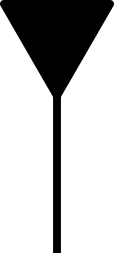
\includegraphics[width=.6cm]{clou_droit.png} & 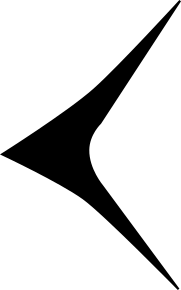
\includegraphics[width=.95cm]{chevron.png} \\\hline
Valeur & 1 & 10 \\
\end{tabular}
\end{center}

Ils utilisent un système sexagésimale (base $60$) et une numération de position. Suivant la place qu'occupe le symbole, celui-ci correspond soit à une unité, soit à une soixantaine ($60$), soit à une soixantaine de soixantaines ($60\times60=3\,600$). On utilise encore aujourd'hui un système sexagésimale pour les unités de temps et des mesures d'angles.\\

Exemples :
\begin{center}
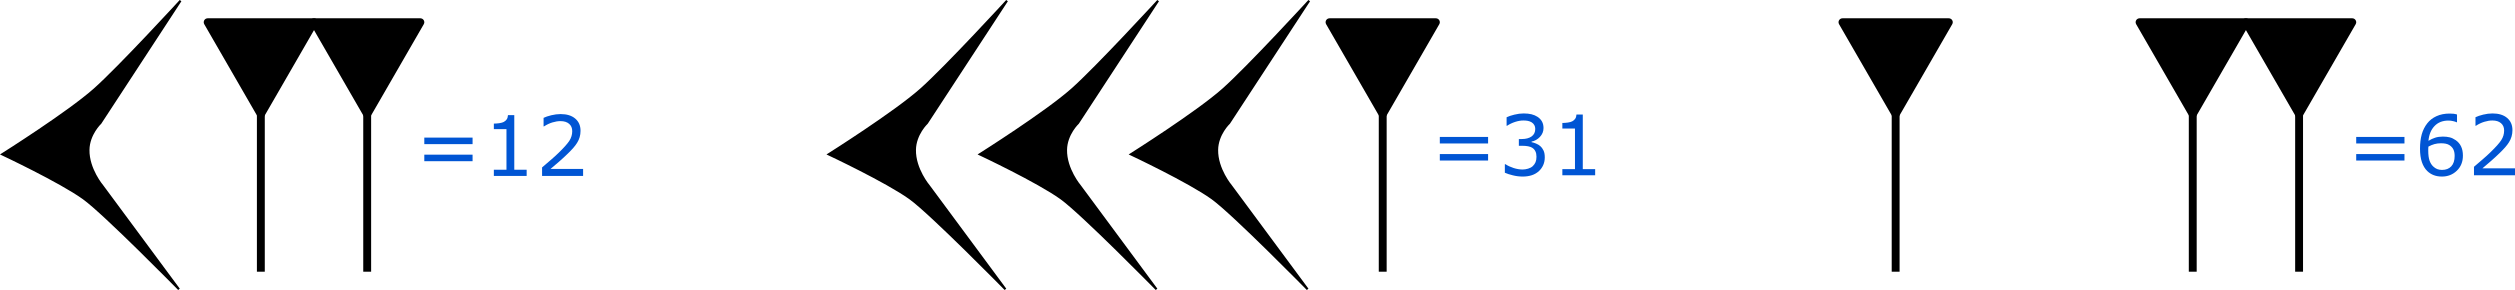
\includegraphics[width=9cm]{exemple_babylonian.png}
\end{center}
\end{His}

\subsection{La numération Égyptienne}

\begin{His}
Au \RNum{3}e millénaire avant J.C., en Egypte, les scribes écrivent les nombres sur des papyrus sous forme de hiéroglyphes. Les égyptiens utilisent un système de numération basé sur le principe additif. Les égyptiens peuvent écrire des nombres entiers jusqu'à $1\,000\,000$. Ils écrivent aussi des nombres décimaux et des fractions.

\newcommand{\egmil}[1]{\multido{\i=1+1}{#1}{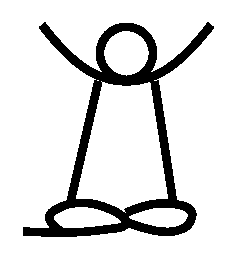
\includegraphics[scale=.1]{egyptian/egypt_person.eps}\hspace{0.5mm}}}
\newcommand{\eghuntho}[1]{\multido{\i=1+1}{#1}{
\includegraphics[scale=.1]{egyptian/egypt_fish.eps}\hspace{0.5mm}}}
\newcommand{\egtentho}[1]{\multido{\i=1+1}{#1}{
\includegraphics[scale=.1]{egyptian/egypt_finger.eps}\hspace{0.5mm}}}
\newcommand{\egtho}[1]{\multido{\i=1+1}{#1}{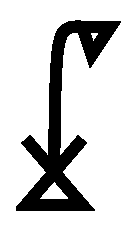
\includegraphics[scale=.1]{egyptian/egypt_lotus.eps}\hspace{0.5mm}}}
\newcommand{\eghun}[1]{\multido{\i=1+1}{#1}{
\includegraphics[scale=.1]{egyptian/egypt_scroll.eps}\hspace{0.5mm}}}
\newcommand{\egten}[1]{\multido{\i=1+1}{#1}{
\includegraphics[scale=.1]{egyptian/egypt_heel.eps}\hspace{0.5mm}}}
\newcommand{\egone}[1]{\multido{\i=1+1}{#1}{
\includegraphics[scale=.1]{egyptian/egypt_stroke.eps}\hspace{0.5mm}}}
\newcommand{\egyptify}[7]{
 \multido{\i=1+1}{#1}{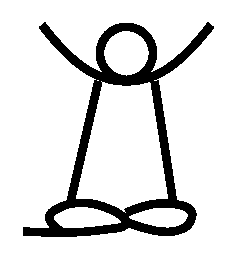
\includegraphics[scale=.1]{egyptian/egypt_person.eps}\hspace{0.5mm}}
 \multido{\i=1+1}{#2}{
\includegraphics[scale=.1]{egyptian/egypt_fish.eps}\hspace{0.5mm}}
 \multido{\i=1+1}{#3}{
\includegraphics[scale=.1]{egyptian/egypt_finger.eps}\hspace{0.5mm}}
 \multido{\i=1+1}{#4}{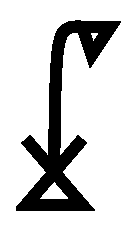
\includegraphics[scale=.1]{egyptian/egypt_lotus.eps}\hspace{0.5mm}}
 \multido{\i=1+1}{#5}{
\includegraphics[scale=.1]{egyptian/egypt_scroll.eps}\hspace{0.5mm}}
 \multido{\i=1+1}{#6}{
\includegraphics[scale=.1]{egyptian/egypt_heel.eps}\hspace{0.5mm}}
 \multido{\i=1+1}{#7}{
\includegraphics[scale=.1]{egyptian/egypt_stroke.eps}\hspace{0.5mm}}
 \hspace{.5mm}
}

\begin{center}
\begin{tabular}[t]{c|c|c|c|c|c|c}
\egmil{1}&\eghuntho{1}&\egtentho{1}&\egtho{1}&\eghun{1}&\egten{1}&\egone{1}\\
\hline
1,000,000&100,000&10,000&1,000&100&10&1\\
\end{tabular}\\
\end{center}

Exemple :

\begin{center}
\egyptify{5}{8}{6}{7}{9}{3}{4}$=5\,867\,934$
\end{center}
\end{His}

\subsection{La numération Maya}

\begin{His}
Dans leur étude des astres, les mayas se servent des nombres pour calculer le temps. Ce sont les inventeurs du calendrier.

 Leur système de numération datant du \RNum{5}e siècle après J.C. suit le principe de position dans la base vigésimale (base $20$). Celui-ci trouve ses origines avec nos $10$ doigts et $10$ orteils !  
 
 Les symboles employés (les glyphes) représentent les nombres jusqu'à $19$, empilés sur différents niveaux. Chaque niveau correspond à un nombre de paquets de $20$ puis de $20\times20=400$ puis de $20\times20\times20=8\,000$...
 
Les mayas utilisent le zéro qu'ils représentent par un coquillage.

\begin{center}
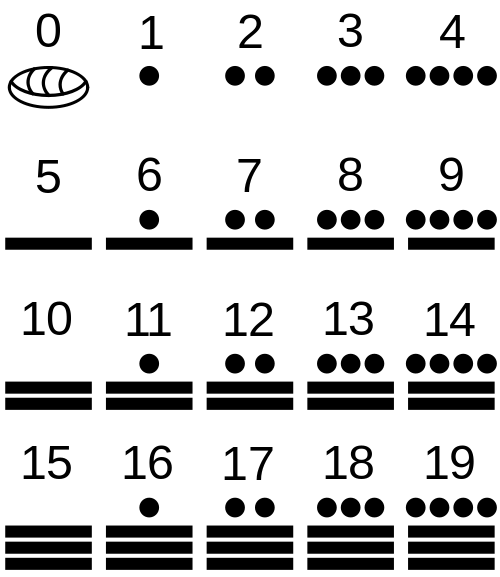
\includegraphics[width=8cm]{maya_numerals.png}
\end{center}

Exemple : $379=18\times20+19$
\begin{center}
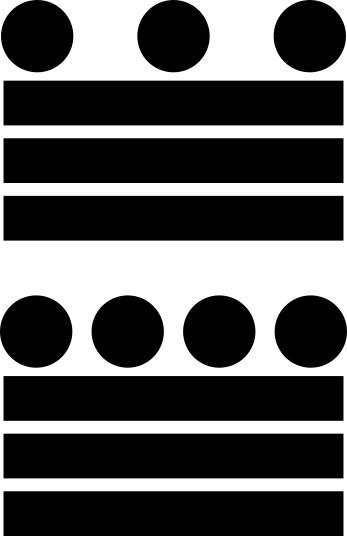
\includegraphics[width=1cm]{maya_exemple.png}
\end{center}
\end{His}

\subsection{La numération Romaine}

\begin{His}
Les grecs et les romains ont inventé des systèmes de numération alphabétiques très peu adaptés aux calculs.

Le système romain est composé de symboles notés côte à côte selon le principe additif et combine les bases $5$ et $10$.

Les plus anciens sont les signes \RNum{1}, \RNum{5}, et \RNum{10} qui dérivent directement de la pratique de l'entaille.

\begin{center}
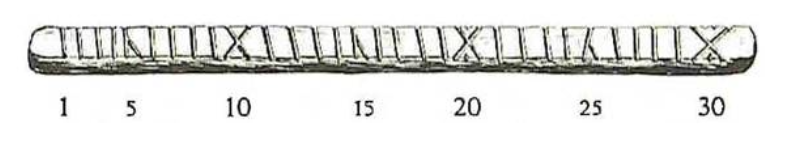
\includegraphics[width=8cm]{roman.png}
\end{center}

\begin{center}
\RNum{1}$=1$\hspace{.5cm}\RNum{2}$=2$\hspace{.5cm}\RNum{3}$=3$\hspace{.5cm}\RNum{4}$=4$\hspace{.5cm}\RNum{5}$=5$\\
\RNum{6}$=6$\hspace{.5cm}\RNum{7}$=7$\hspace{.5cm}\RNum{8}$=8$\hspace{.5cm}\RNum{9}$=9$\hspace{.5cm}\RNum{10}$=10$\\
\RNum{20}$=20$\hspace{.5cm}\RNum{50}$=50$\hspace{.5cm}\RNum{100}$=100$\hspace{.5cm}\RNum{500}$=500$\hspace{.5cm}\RNum{1000}$=1000$
\end{center}

Exemple :
\begin{center}
\RNum{6963}$=6\,963$
\end{center}
\end{His}

\subsection{L'histoire de nos chiffres}

\begin{His}
Nos chiffres de "$1$" à "$9$" que nous appelons à tort "chiffres arabes", viennent en réalité des Indes. Leurs "ancêtres" les plus anciens apparaissent dans des inscriptions des grottes de Nana Ghât datant du \RNum{2}e siècle avant J.C.

Au \RNum{5}e siècle de notre ère, en Inde, les savants ont l'idée ingénieuse de marier le principe de position, les neuf symboles et les zéro en tant que nombre à part entière représentant une quantité qui n'existe pas.

\begin{center}

\includegraphics[width=10cm]{indian1.png}\\
\textbf{Numération indienne}
\end{center}

Au \RNum{8}e siècle après J.C., alors que l'islam s'étend sur une partie de l'Afrique et de l'Asie, les califes de Bagdad font traduire les œuvres majeurs des peuples sur lesquels ils règnent.

Parmi elles se trouve l'œuvre de Brahmagupta, un mathématicien indien. Sa numération à dix chiffres est si ingénieuse que les marchands arabes l'adoptent immédiatement.

\begin{center}

\includegraphics[width=10cm]{indian2.png}\\
\textbf{Numération arabe}
\end{center}
\end{His}

\begin{His}
Au \RNum{9}e siècle, les chiffres arabes sont décrits dans un ouvrage du mathématicien et astronome Muhammad ibn Musa el-Khwarizmi ($790-850$) qui, traduit en latin, les diffuse en Espagne.\\

Gerbert d'Aurillac ($945-1003$) qui deviendra pape en $999$, est passionné par les mathématiques. Il rédige deux traités, l'un sur la multiplication, l'autre sur la division. Il initiera pour la première fois l'occident chrétien aux chiffres "indo-arabes" mais il ne retient ni la numération de position ni le zéro. 

\begin{center}

\includegraphics[width=10cm]{indian3.png}\\
\textbf{Numération hispano-arabe}
\end{center}

Au \RNum{13}e siècle, le mathématicien italien Léonard de Pise ($1175-1250$), dit Fibonacci publia, en $1202$, le \textit{Liber Abaci} (le livre du calcul), un traité sur les calculs et la comptabilité fondée sur le calcul décimal.\\

Au \RNum{15}e siècle, avec l'expansion de l'imprimerie, les chiffres ont été légèrement déformés pour donner une forme semblable à la forme actuelle. 

\begin{center}

\includegraphics[width=10cm]{indian4.png}\\
\textbf{Numération italienne}
\end{center}
\end{His}
